Underwater imaging has long been crucial in various fields, from marine research to environmental monitoring, underwater archaeology, and offshore industries. For example, scientists use underwater photography with quadrats to audit the abundance of coral over time at several reef locations or to examine phenomena such as hydrothermal vents, underwater volcanic eruptions and gas seepages from the seafloor \cite{universityofhawaiiPracticesScienceUnderwater}. Unmanned Underwater Vehicles (UUVs), a type of submersible vehicle, are pivotal in advancing underwater imaging capabilities. These autonomous or remotely operated vehicles, often housing vast arrays of sophisticated sensors, enable the end user to explore and analyse underwater environments with unprecedented accuracy and efficiency. Their autonomous or remote-controlled nature advocates the ideal platform for conducting missions of extended duration in hazardous conditions, impossible for direct human presence and intervention. With the benefits of UUV deployment, they have become common as a safer and cheaper alternative to manned vehicular operations in the vast range of underwater imaging-related industries and applications, such as intelligence surveillance and reconnaissance in defence, inspection and identification of defects or foreign objects in maritime, and oceanography and hydrography in marine research \cite{yannickallardUnmannedUnderwaterVehicle2014}.

\begin{figure}[h]
    \centering
    \begin{subfigure}{.49\textwidth}
        \centering
        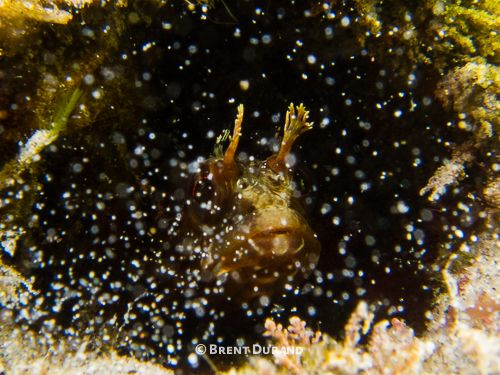
\includegraphics[width=1\linewidth]{assets/backscatter_article_durand2.jpg}
        \caption{}
        \label{subfig:backscatter_durand}
    \end{subfigure}
    \hfill
    \begin{subfigure}{.49\textwidth}
        \centering
        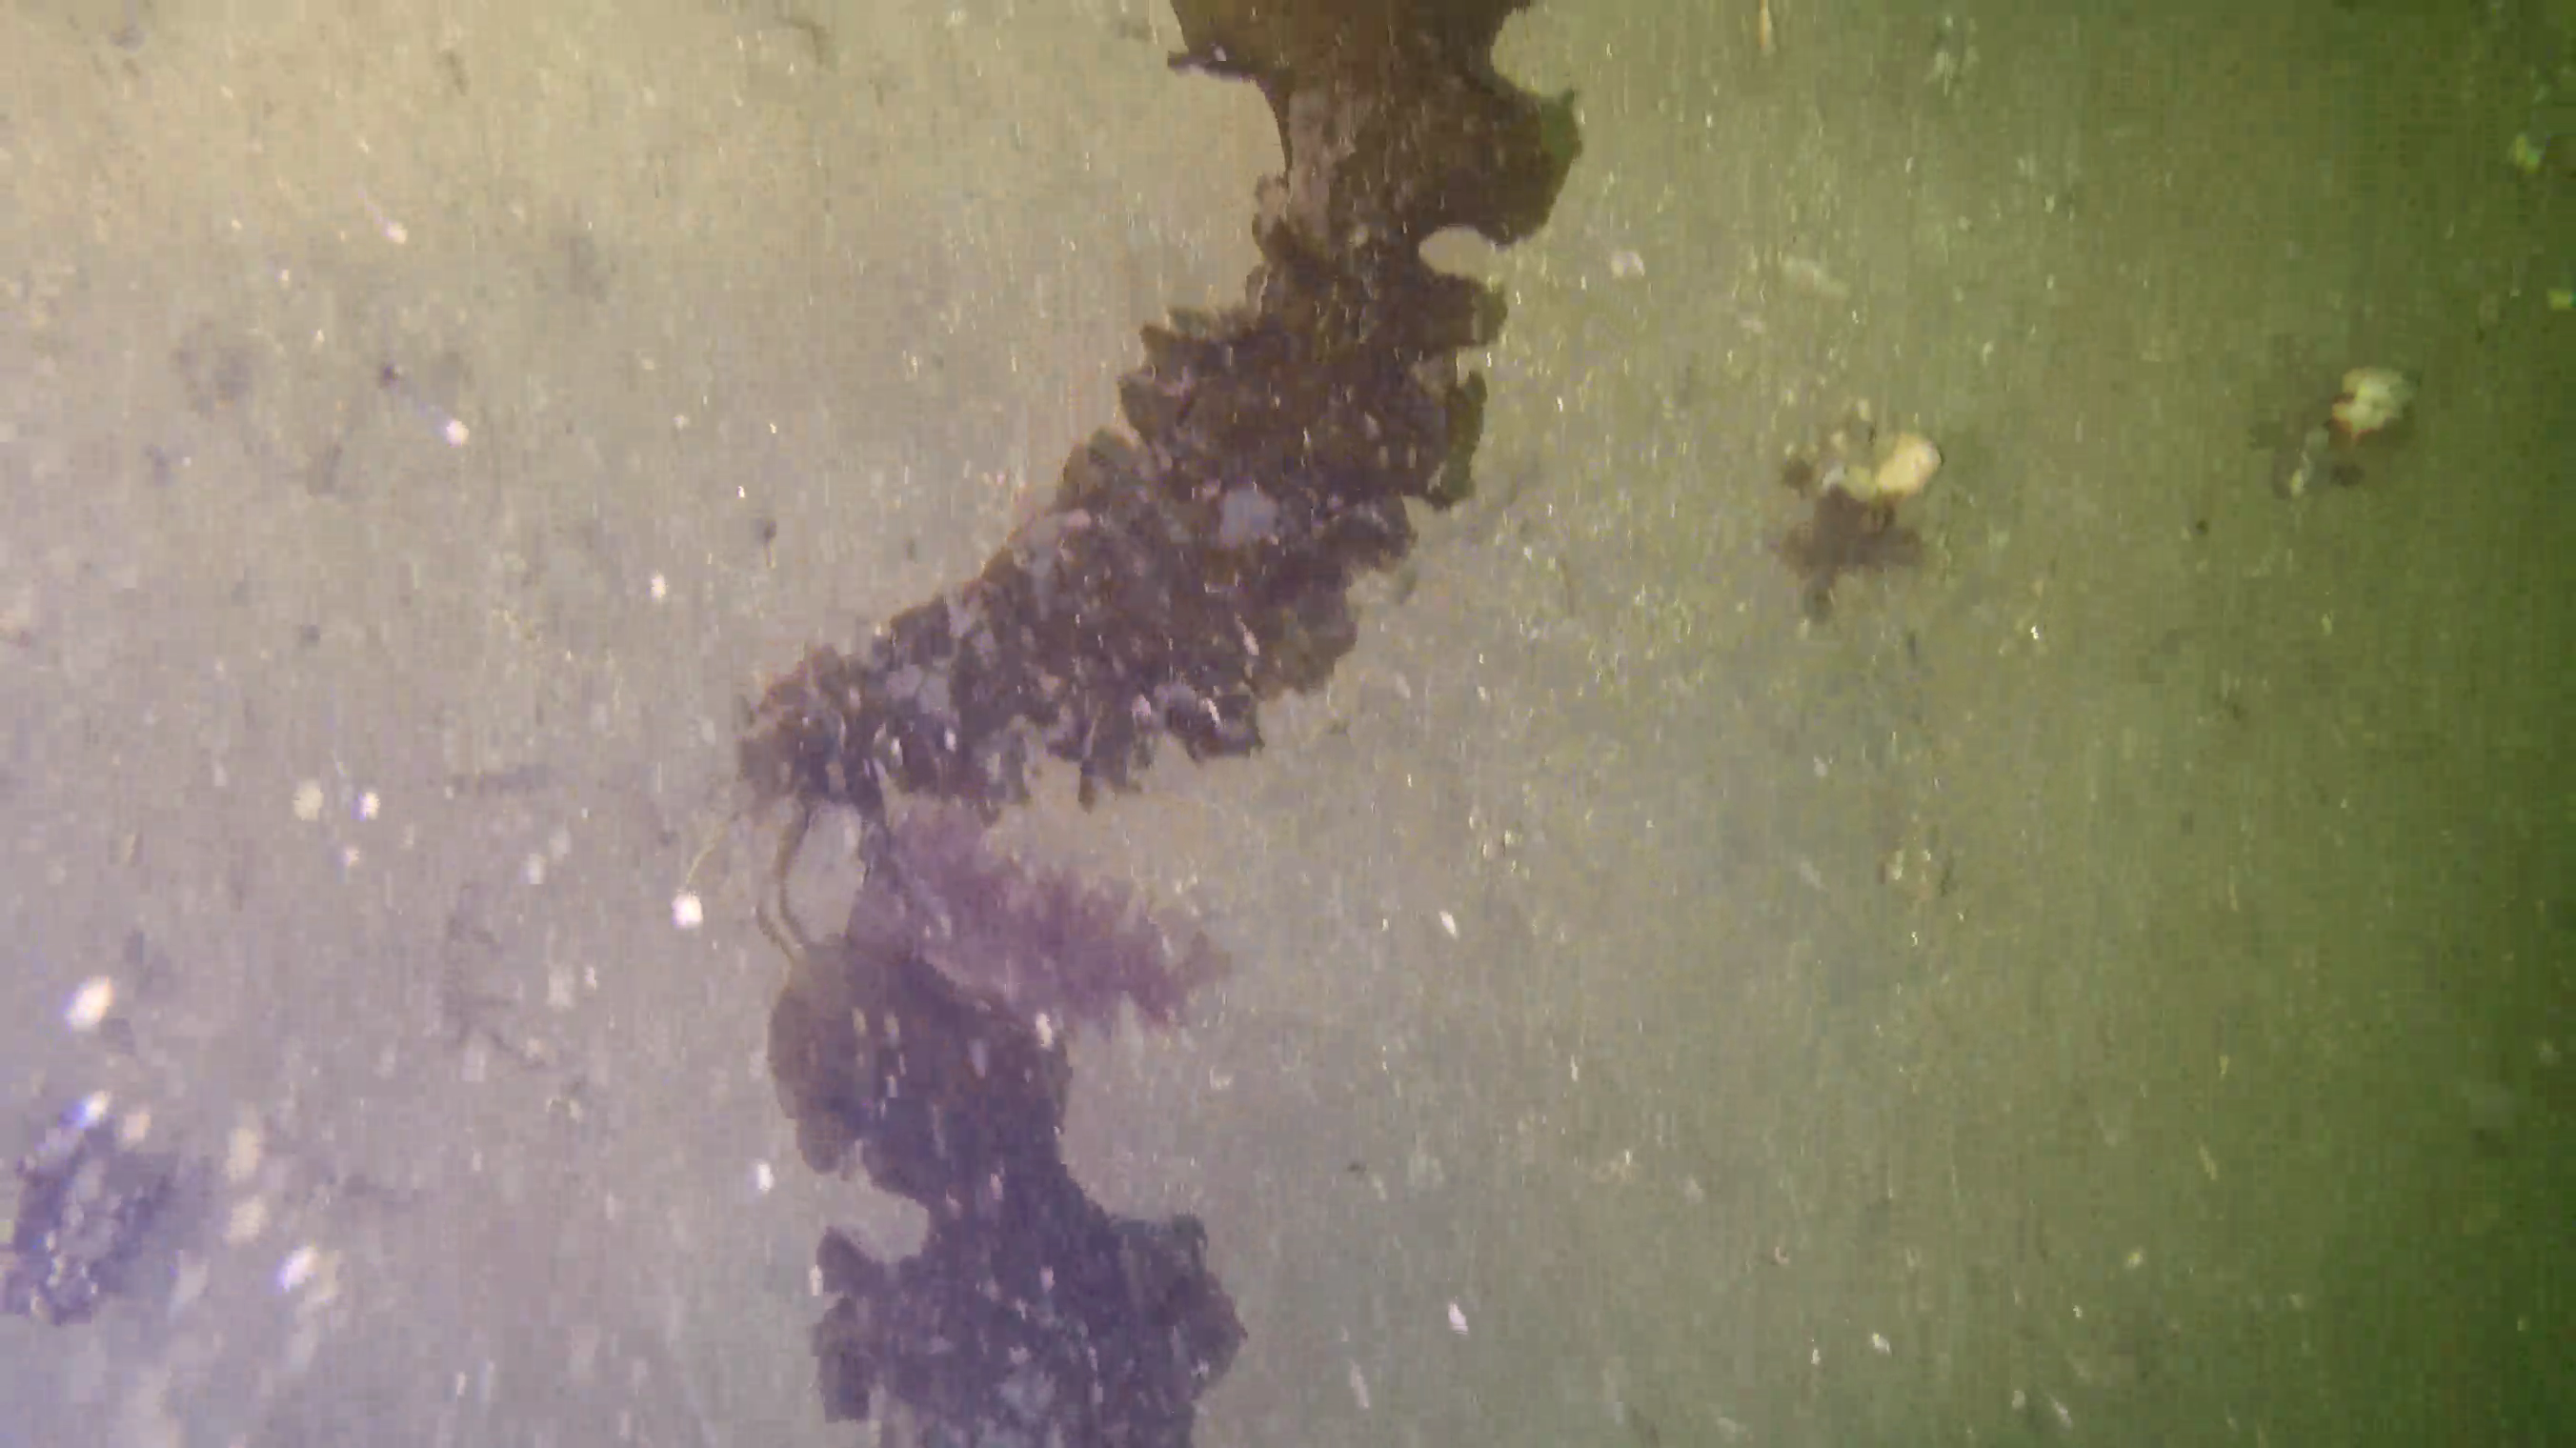
\includegraphics[width=1\linewidth]{assets/backscatter_test_vid.png}
        \caption{}
        \label{subfig:backscatter_gopro}
    \end{subfigure}
    \caption{(a) Backscatter is formed as the particles of sand drift between the aquatic animal and the camera \cite{brentdurandEasyWaysEliminate2013}. (b) A captured frame in GoPro footage from a UUV of the seabed with backscatter formed as the propellors disrupt the sand.}
    \label{fig:backscatter}
\end{figure}

Despite its importance, underwater imaging faces numerous challenges that hinder its effectiveness, from developing an air-tight camera housing to working around the lack of light attenuation at greater sea depths. An external high-power light source is often tied to a camera to ensure a well-lit imaging scene. However, this produces the most sovereign of all challenges: backscatter, shown in Figure \ref{fig:backscatter}, where suspended particles in water scatter light in an inhomogeneous manner. The most detrimental form of backscatter originates from particles reflecting the light emitted by the light source back into the camera, creating exponentially bright spots and often saturating the image and degrading the quality. Universal techniques exist to eliminate backscatter in underwater imaging \cite{brentdurandEasyWaysEliminate2013}: (a) Reduce the space between the camera and the subject to lower the number of backscatter particles in the space between, (b) Fine-tune the light source positioning by altering the angle such that only the edge of the light cone illuminates the subject without illuminating the space in front of the camera, (c) By achieving perfect buoyancy, a diver can minimise creating clouds of sand and debris when ensuring stability underwater. While these techniques are straightforward, they lack viability for UUVs due to the erratic backscatter formation from the continuous and arbitrary motion of the propellors and general vehicular movement.

The ultimate goal of this project is to develop a cutting-edge light source system capable of aiding the generation of high-quality underwater images, mainly the seafloor, from UUVs without backscatter interference. Achieving this ambitious goal requires a multi-disciplinary approach encompassing efficient machine vision technologies and innovative hardware integration. This project first aims to research systems and develop reliable backscatter detection and elimination capabilities, with a specialised projector serving as a dynamic light source of tailored light patterns for selective scene illumination to mitigate backscatter effects. The second research aim will look into architectures and methodologies to optimise the system for real-time to ensure adherence to stringent requirements for predictability, stability, efficiency, and reliability, ultimately allowing for control of computational parameters to maximise imaging performance in dynamic underwater environments whilst maintaining requirements. The final research aim is delving into the engineering of a predictive system for anticipating the future positions of detected backscatter particles, enabling proactive elimination strategies without the need for continuous, computationally intensive machine vision processing, for efficient and preemptive adjustments to the light projection patterns for optimal backscatter suppression. These three aims represent critical trade-offs that must be carefully balanced to achieve the overarching objective, which this research project aims to establish through systematic exploration and optimisation to lead towards a novel framework for enhancing underwater imaging capabilities.
